% Options for packages loaded elsewhere
\PassOptionsToPackage{unicode}{hyperref}
\PassOptionsToPackage{hyphens}{url}
%
\documentclass[
]{article}
\usepackage{amsmath,amssymb}
\usepackage{lmodern}
\usepackage{iftex}
\ifPDFTeX
  \usepackage[T1]{fontenc}
  \usepackage[utf8]{inputenc}
  \usepackage{textcomp} % provide euro and other symbols
\else % if luatex or xetex
  \usepackage{unicode-math}
  \defaultfontfeatures{Scale=MatchLowercase}
  \defaultfontfeatures[\rmfamily]{Ligatures=TeX,Scale=1}
\fi
% Use upquote if available, for straight quotes in verbatim environments
\IfFileExists{upquote.sty}{\usepackage{upquote}}{}
\IfFileExists{microtype.sty}{% use microtype if available
  \usepackage[]{microtype}
  \UseMicrotypeSet[protrusion]{basicmath} % disable protrusion for tt fonts
}{}
\makeatletter
\@ifundefined{KOMAClassName}{% if non-KOMA class
  \IfFileExists{parskip.sty}{%
    \usepackage{parskip}
  }{% else
    \setlength{\parindent}{0pt}
    \setlength{\parskip}{6pt plus 2pt minus 1pt}}
}{% if KOMA class
  \KOMAoptions{parskip=half}}
\makeatother
\usepackage{xcolor}
\usepackage[margin=1in]{geometry}
\usepackage{color}
\usepackage{fancyvrb}
\newcommand{\VerbBar}{|}
\newcommand{\VERB}{\Verb[commandchars=\\\{\}]}
\DefineVerbatimEnvironment{Highlighting}{Verbatim}{commandchars=\\\{\}}
% Add ',fontsize=\small' for more characters per line
\usepackage{framed}
\definecolor{shadecolor}{RGB}{248,248,248}
\newenvironment{Shaded}{\begin{snugshade}}{\end{snugshade}}
\newcommand{\AlertTok}[1]{\textcolor[rgb]{0.94,0.16,0.16}{#1}}
\newcommand{\AnnotationTok}[1]{\textcolor[rgb]{0.56,0.35,0.01}{\textbf{\textit{#1}}}}
\newcommand{\AttributeTok}[1]{\textcolor[rgb]{0.77,0.63,0.00}{#1}}
\newcommand{\BaseNTok}[1]{\textcolor[rgb]{0.00,0.00,0.81}{#1}}
\newcommand{\BuiltInTok}[1]{#1}
\newcommand{\CharTok}[1]{\textcolor[rgb]{0.31,0.60,0.02}{#1}}
\newcommand{\CommentTok}[1]{\textcolor[rgb]{0.56,0.35,0.01}{\textit{#1}}}
\newcommand{\CommentVarTok}[1]{\textcolor[rgb]{0.56,0.35,0.01}{\textbf{\textit{#1}}}}
\newcommand{\ConstantTok}[1]{\textcolor[rgb]{0.00,0.00,0.00}{#1}}
\newcommand{\ControlFlowTok}[1]{\textcolor[rgb]{0.13,0.29,0.53}{\textbf{#1}}}
\newcommand{\DataTypeTok}[1]{\textcolor[rgb]{0.13,0.29,0.53}{#1}}
\newcommand{\DecValTok}[1]{\textcolor[rgb]{0.00,0.00,0.81}{#1}}
\newcommand{\DocumentationTok}[1]{\textcolor[rgb]{0.56,0.35,0.01}{\textbf{\textit{#1}}}}
\newcommand{\ErrorTok}[1]{\textcolor[rgb]{0.64,0.00,0.00}{\textbf{#1}}}
\newcommand{\ExtensionTok}[1]{#1}
\newcommand{\FloatTok}[1]{\textcolor[rgb]{0.00,0.00,0.81}{#1}}
\newcommand{\FunctionTok}[1]{\textcolor[rgb]{0.00,0.00,0.00}{#1}}
\newcommand{\ImportTok}[1]{#1}
\newcommand{\InformationTok}[1]{\textcolor[rgb]{0.56,0.35,0.01}{\textbf{\textit{#1}}}}
\newcommand{\KeywordTok}[1]{\textcolor[rgb]{0.13,0.29,0.53}{\textbf{#1}}}
\newcommand{\NormalTok}[1]{#1}
\newcommand{\OperatorTok}[1]{\textcolor[rgb]{0.81,0.36,0.00}{\textbf{#1}}}
\newcommand{\OtherTok}[1]{\textcolor[rgb]{0.56,0.35,0.01}{#1}}
\newcommand{\PreprocessorTok}[1]{\textcolor[rgb]{0.56,0.35,0.01}{\textit{#1}}}
\newcommand{\RegionMarkerTok}[1]{#1}
\newcommand{\SpecialCharTok}[1]{\textcolor[rgb]{0.00,0.00,0.00}{#1}}
\newcommand{\SpecialStringTok}[1]{\textcolor[rgb]{0.31,0.60,0.02}{#1}}
\newcommand{\StringTok}[1]{\textcolor[rgb]{0.31,0.60,0.02}{#1}}
\newcommand{\VariableTok}[1]{\textcolor[rgb]{0.00,0.00,0.00}{#1}}
\newcommand{\VerbatimStringTok}[1]{\textcolor[rgb]{0.31,0.60,0.02}{#1}}
\newcommand{\WarningTok}[1]{\textcolor[rgb]{0.56,0.35,0.01}{\textbf{\textit{#1}}}}
\usepackage{graphicx}
\makeatletter
\def\maxwidth{\ifdim\Gin@nat@width>\linewidth\linewidth\else\Gin@nat@width\fi}
\def\maxheight{\ifdim\Gin@nat@height>\textheight\textheight\else\Gin@nat@height\fi}
\makeatother
% Scale images if necessary, so that they will not overflow the page
% margins by default, and it is still possible to overwrite the defaults
% using explicit options in \includegraphics[width, height, ...]{}
\setkeys{Gin}{width=\maxwidth,height=\maxheight,keepaspectratio}
% Set default figure placement to htbp
\makeatletter
\def\fps@figure{htbp}
\makeatother
\setlength{\emergencystretch}{3em} % prevent overfull lines
\providecommand{\tightlist}{%
  \setlength{\itemsep}{0pt}\setlength{\parskip}{0pt}}
\setcounter{secnumdepth}{-\maxdimen} % remove section numbering
\ifLuaTeX
  \usepackage{selnolig}  % disable illegal ligatures
\fi
\IfFileExists{bookmark.sty}{\usepackage{bookmark}}{\usepackage{hyperref}}
\IfFileExists{xurl.sty}{\usepackage{xurl}}{} % add URL line breaks if available
\urlstyle{same} % disable monospaced font for URLs
\hypersetup{
  pdftitle={Creating maps in R - basics},
  pdfauthor={Heidi Rautiainen},
  hidelinks,
  pdfcreator={LaTeX via pandoc}}

\title{Creating maps in R - basics}
\author{Heidi Rautiainen}
\date{2024-12-20, Updated: 2026-01-21}

\begin{document}
\maketitle

\hypertarget{set-up-directory-install-packages-and-load-packages}{%
\section{Set up directory, install packages and load
packages}\label{set-up-directory-install-packages-and-load-packages}}

\hypertarget{exercise-1-create-study-area-map-using-ggplot}{%
\section{Exercise 1: Create study area map using
``ggplot''}\label{exercise-1-create-study-area-map-using-ggplot}}

All datasets are found in the ``data''-folder.

Here, we use the package `rnaturalearth' to download countries in a ESRI
shapefile format. These are available for download here:
\url{https://www.naturalearthdata.com/downloads/10m-cultural-vectors/10m-admin-0-countries/}

\textbf{Coordinate reference systems (CRS)}\\
CRS provide a standardized way of describing locations to describe
geographic data. The CRS that is chosen depends on when the data was
collected, the purpose of the data, etc. It is necessary to transform
vector and raster data to a common CRS when data with different CRS are
combined.

\textbf{\emph{Setting CRS to SWEREF99 (Sweden). CRS can be referenced by
its:}}

\begin{enumerate}
\def\labelenumi{\arabic{enumi}.}
\item
  EPSG code, CRS(``+init=epsg:3006'') (see
  \url{http://www.epsg-registry.org/} and
  \url{http://spatialreference.org/}) or by
\item
  proj4spring; ``+proj=utm +zone=33 +ellps=GRS80 +towgs84=0,0,0,0,0,0,0
  +units=m +no\_defs''
\end{enumerate}

\textbf{\emph{There are two general options:}}

\begin{enumerate}
\def\labelenumi{\arabic{enumi}.}
\item
  unprojected (a.k.a. Geographic): Latitude/Longitude for referencing
  location on the ellipsoid Earth (wgs84), and
\item
  projected: Easting/Northing for referencing location on 2D
  representations of Earth (the creation of maps) e.g., SWEREF99.
\end{enumerate}

More reading:\\
\url{https://www.nceas.ucsb.edu/sites/default/files/2020-04/OverviewCoordinateReferenceSystems.pdf}

\hypertarget{load-vector-data}{%
\subsection{Load vector data}\label{load-vector-data}}

How to download using ``rnaturalearth'' and save the shp locally

I will open the saved .shp for the exercise:

\begin{Shaded}
\begin{Highlighting}[]
\DocumentationTok{\#\# load country boarders {-}{-}{-}{-}{-}{-}{-}{-}{-}{-}{-}}


\CommentTok{\#\textquotesingle{} downladed and saved from rnaturalearth (above)}
\NormalTok{swe\_no\_sweref }\OtherTok{\textless{}{-}}\NormalTok{  input\_vector }\SpecialCharTok{\%\textgreater{}\%} 

  \CommentTok{\# value = T: return vector containing the matching elements}
  \FunctionTok{grep}\NormalTok{(}\AttributeTok{pattern =} \StringTok{"swe\_no"}\NormalTok{, }\AttributeTok{value =}\NormalTok{ T) }\SpecialCharTok{\%\textgreater{}\%} 

  \CommentTok{\# read ESRI Shapefile object }
\NormalTok{  sf}\SpecialCharTok{::}\FunctionTok{st\_read}\NormalTok{() }\SpecialCharTok{\%\textgreater{}\%} 

  \CommentTok{\#convert geometry object into an sf object}
  \FunctionTok{st\_as\_sf}\NormalTok{() }
\end{Highlighting}
\end{Shaded}

\begin{verbatim}
## Reading layer `swe_no' from data source 
##   `/Users/hirn0001/Library/CloudStorage/OneDrive-Sverigeslantbruksuniversitet/Undervisning/Teaching and courses/GS_VMAS Data handling and illustrations/2025/create-maps/input_data/vector/country/swe_no.shp' 
##   using driver `ESRI Shapefile'
## Simple feature collection with 2 features and 168 fields
## Geometry type: MULTIPOLYGON
## Dimension:     XY
## Bounding box:  xmin: -362704.5 ymin: -6097519 xmax: 1114145 ymax: 8972413
## Projected CRS: SWEREF99 TM
\end{verbatim}

\begin{Shaded}
\begin{Highlighting}[]
\CommentTok{\# check coordinate system }
\FunctionTok{st\_crs}\NormalTok{(swe\_no\_sweref)}\SpecialCharTok{$}\NormalTok{proj4string}
\end{Highlighting}
\end{Shaded}

\begin{verbatim}
## [1] "+proj=utm +zone=33 +ellps=GRS80 +towgs84=0,0,0,0,0,0,0 +units=m +no_defs"
\end{verbatim}

\begin{Shaded}
\begin{Highlighting}[]
\CommentTok{\# Create a bounding box as an sf object for layers {-}{-}{-}{-}}
\NormalTok{b\_box }\OtherTok{\textless{}{-}} \FunctionTok{c}\NormalTok{(}\AttributeTok{xmin =} \DecValTok{350432}\NormalTok{, }\AttributeTok{ymin =} \DecValTok{7179284}\NormalTok{, }
           \AttributeTok{xmax =} \DecValTok{857780}\NormalTok{, }\AttributeTok{ymax =}\DecValTok{7444230}\NormalTok{)}

\CommentTok{\# Now intersect the full world\textquotesingle{}s coastline with the bounding box }
\FunctionTok{suppressWarnings}\NormalTok{(\{ }
\NormalTok{sweden.c }\OtherTok{\textless{}{-}} \FunctionTok{st\_crop}\NormalTok{(swe\_no\_sweref, b\_box)}
\FunctionTok{plot}\NormalTok{(sweden.c)}
\NormalTok{\}) }
\end{Highlighting}
\end{Shaded}

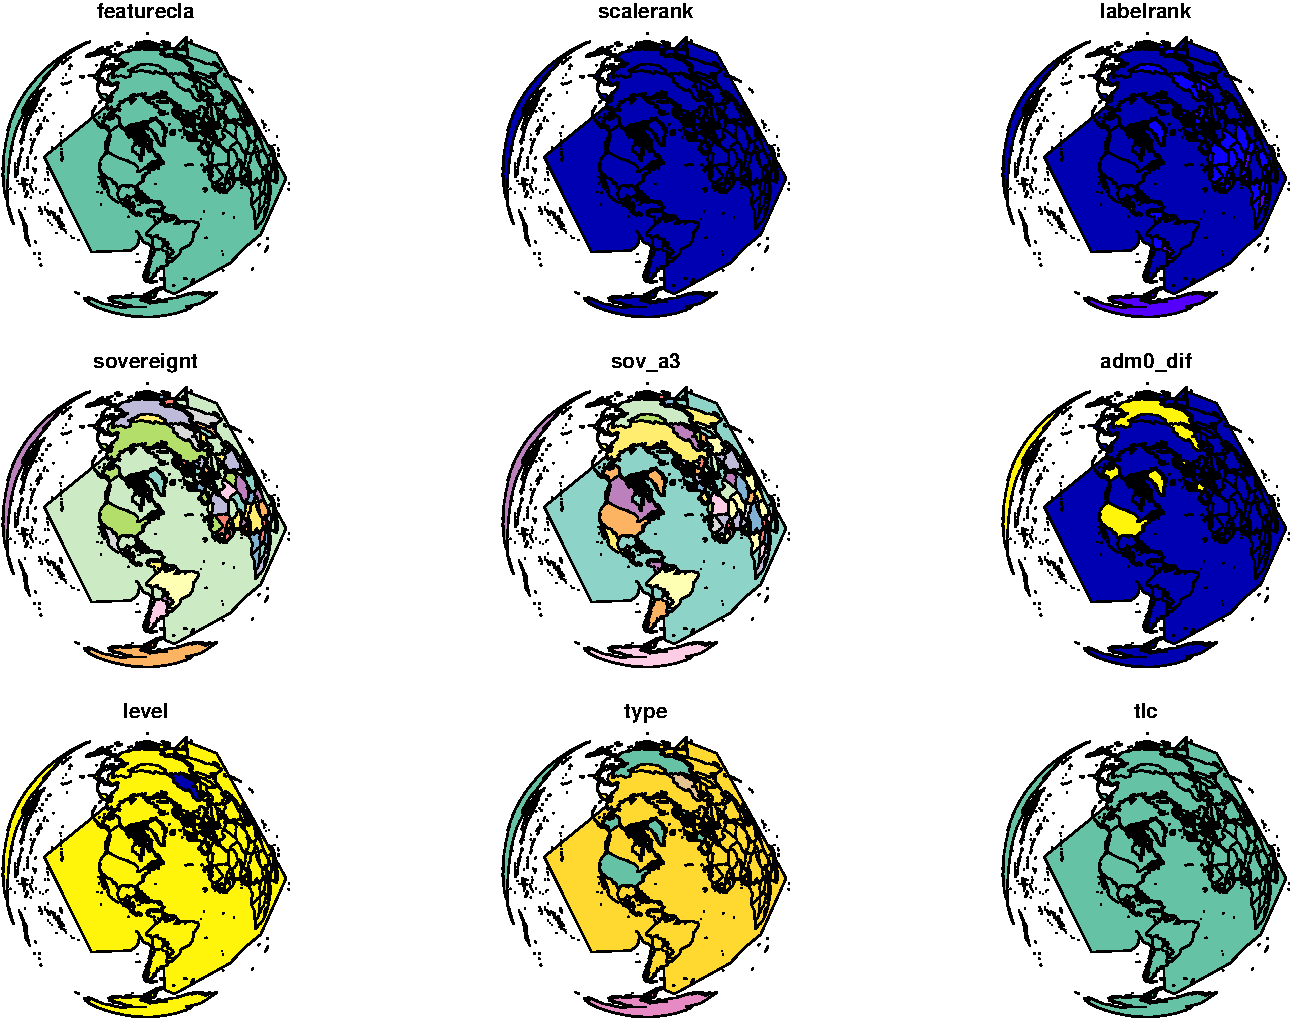
\includegraphics{Tutorial_files/figure-latex/unnamed-chunk-2-1.pdf}

\begin{Shaded}
\begin{Highlighting}[]
\FunctionTok{class}\NormalTok{(sweden.c)}
\end{Highlighting}
\end{Shaded}

\begin{verbatim}
## [1] "sf"         "data.frame"
\end{verbatim}

\begin{Shaded}
\begin{Highlighting}[]
\DocumentationTok{\#\#\# water data {-}{-}{-}{-}}
\NormalTok{input\_vector}
\end{Highlighting}
\end{Shaded}

\begin{verbatim}
## [1] "input_data/vector/animal_data/data_cleaned_PV.rds"                                      
## [2] "input_data/vector/animal_data/data_ready_rsf.rds"                                       
## [3] "input_data/vector/animal_data/reindeer_data.rds"                                        
## [4] "input_data/vector/country/swe_no.shp"                                                   
## [5] "input_data/vector/country/swe.shp"                                                      
## [6] "input_data/vector/HR/spatial_files_availability_PV_winter_2021_shorter_modified_new.shp"
## [7] "input_data/vector/ne_10m_lakes/ne_10m_lakes.shp"
\end{verbatim}

\begin{Shaded}
\begin{Highlighting}[]
\CommentTok{\# import lakes}
\NormalTok{lakes }\OtherTok{\textless{}{-}}\NormalTok{  input\_vector }\SpecialCharTok{\%\textgreater{}\%}
  \FunctionTok{grep}\NormalTok{(}\AttributeTok{pattern =} \StringTok{"lakes"}\NormalTok{, }\AttributeTok{value =}\NormalTok{ T) }\SpecialCharTok{\%\textgreater{}\%}
\NormalTok{  sf}\SpecialCharTok{::}\FunctionTok{st\_read}\NormalTok{() }\SpecialCharTok{\%\textgreater{}\%}
  \FunctionTok{st\_as\_sf}\NormalTok{() }
\end{Highlighting}
\end{Shaded}

\begin{verbatim}
## Reading layer `ne_10m_lakes' from data source 
##   `/Users/hirn0001/Library/CloudStorage/OneDrive-Sverigeslantbruksuniversitet/Undervisning/Teaching and courses/GS_VMAS Data handling and illustrations/2025/create-maps/input_data/vector/ne_10m_lakes/ne_10m_lakes.shp' 
##   using driver `ESRI Shapefile'
## Simple feature collection with 1355 features and 41 fields
## Geometry type: MULTIPOLYGON
## Dimension:     XY
## Bounding box:  xmin: -165.9656 ymin: -50.66967 xmax: 177.1544 ymax: 81.95521
## Geodetic CRS:  WGS 84
\end{verbatim}

\begin{Shaded}
\begin{Highlighting}[]
\FunctionTok{class}\NormalTok{(lakes)}
\end{Highlighting}
\end{Shaded}

\begin{verbatim}
## [1] "sf"         "data.frame"
\end{verbatim}

\begin{Shaded}
\begin{Highlighting}[]
\FunctionTok{st\_crs}\NormalTok{(lakes)}
\end{Highlighting}
\end{Shaded}

\begin{verbatim}
## Coordinate Reference System:
##   User input: WGS 84 
##   wkt:
## GEOGCRS["WGS 84",
##     DATUM["World Geodetic System 1984",
##         ELLIPSOID["WGS 84",6378137,298.257223563,
##             LENGTHUNIT["metre",1]]],
##     PRIMEM["Greenwich",0,
##         ANGLEUNIT["degree",0.0174532925199433]],
##     CS[ellipsoidal,2],
##         AXIS["latitude",north,
##             ORDER[1],
##             ANGLEUNIT["degree",0.0174532925199433]],
##         AXIS["longitude",east,
##             ORDER[2],
##             ANGLEUNIT["degree",0.0174532925199433]],
##     ID["EPSG",4326]]
\end{verbatim}

\begin{Shaded}
\begin{Highlighting}[]
\CommentTok{\# Transform or convert coordinates of simple feature (sf)}
\NormalTok{lakes }\OtherTok{\textless{}{-}} \FunctionTok{st\_transform}\NormalTok{(lakes, }\AttributeTok{crs =} \DecValTok{3006}\NormalTok{) }
\FunctionTok{suppressWarnings}\NormalTok{(\{ }
  
\CommentTok{\# crop an sf object to a specific rectangle (here based on extent of "sweden.c"{-}shp)}
\CommentTok{\# sf\_use\_s2(FALSE) \# use if errors occur below}
\NormalTok{lakes }\OtherTok{\textless{}{-}} \FunctionTok{st\_crop}\NormalTok{(lakes, sweden.c) }

\FunctionTok{class}\NormalTok{(lakes)}
\FunctionTok{plot}\NormalTok{(lakes)}
\NormalTok{\}) }
\end{Highlighting}
\end{Shaded}

\includegraphics{Tutorial_files/figure-latex/unnamed-chunk-2-2.pdf}

\hypertarget{create-points-of-interest-cities}{%
\subsubsection{Create points of interest
(cities)}\label{create-points-of-interest-cities}}

Create xy points with labels. Here creating sf-object and setting the
crs.

\begin{Shaded}
\begin{Highlighting}[]
\CommentTok{\# Create points of interest (coordinates from QGIS or google maps for demonstration)}
\NormalTok{places }\OtherTok{\textless{}{-}} \FunctionTok{data.frame}\NormalTok{(}\AttributeTok{ID=} \FunctionTok{c}\NormalTok{(}\StringTok{"Arjeplog"}\NormalTok{, }\StringTok{"Arvidsjaur"}\NormalTok{, }\StringTok{"Sorsele"}\NormalTok{),}
                     \AttributeTok{y =} \FunctionTok{c}\NormalTok{(}\FloatTok{7328407.945}\NormalTok{, }\FloatTok{7280856.153}\NormalTok{, }\FloatTok{7270326.684}\NormalTok{),}
                     \AttributeTok{x =} \FunctionTok{c}\NormalTok{(}\FloatTok{630040.101}\NormalTok{, }\FloatTok{693262.414}\NormalTok{, }\FloatTok{617477.638}\NormalTok{)) }\SpecialCharTok{\%\textgreater{}\%}
  
  \FunctionTok{st\_as\_sf}\NormalTok{(}\AttributeTok{coords =} \FunctionTok{c}\NormalTok{(}\StringTok{"x"}\NormalTok{, }\StringTok{"y"}\NormalTok{),  }\CommentTok{\# create sf object }
           
           \AttributeTok{crs=}\FunctionTok{st\_crs}\NormalTok{(sweden.c))  }\CommentTok{\# set same crs as for sweden.c     }
\FunctionTok{class}\NormalTok{(places)}
\end{Highlighting}
\end{Shaded}

\begin{verbatim}
## [1] "sf"         "data.frame"
\end{verbatim}

\begin{Shaded}
\begin{Highlighting}[]
 \FunctionTok{st\_crs}\NormalTok{(places) }\CommentTok{\# check projection }
\end{Highlighting}
\end{Shaded}

\begin{verbatim}
## Coordinate Reference System:
##   User input: SWEREF99 TM 
##   wkt:
## PROJCRS["SWEREF99 TM",
##     BASEGEOGCRS["SWEREF99",
##         DATUM["SWEREF99",
##             ELLIPSOID["GRS 1980",6378137,298.257222101,
##                 LENGTHUNIT["metre",1]]],
##         PRIMEM["Greenwich",0,
##             ANGLEUNIT["degree",0.0174532925199433]],
##         ID["EPSG",4619]],
##     CONVERSION["SWEREF99 TM",
##         METHOD["Transverse Mercator",
##             ID["EPSG",9807]],
##         PARAMETER["Latitude of natural origin",0,
##             ANGLEUNIT["degree",0.0174532925199433],
##             ID["EPSG",8801]],
##         PARAMETER["Longitude of natural origin",15,
##             ANGLEUNIT["degree",0.0174532925199433],
##             ID["EPSG",8802]],
##         PARAMETER["Scale factor at natural origin",0.9996,
##             SCALEUNIT["unity",1],
##             ID["EPSG",8805]],
##         PARAMETER["False easting",500000,
##             LENGTHUNIT["metre",1],
##             ID["EPSG",8806]],
##         PARAMETER["False northing",0,
##             LENGTHUNIT["metre",1],
##             ID["EPSG",8807]]],
##     CS[Cartesian,2],
##         AXIS["northing (N)",north,
##             ORDER[1],
##             LENGTHUNIT["metre",1]],
##         AXIS["easting (E)",east,
##             ORDER[2],
##             LENGTHUNIT["metre",1]],
##     USAGE[
##         SCOPE["Topographic mapping (medium and small scale)."],
##         AREA["Sweden - onshore and offshore."],
##         BBOX[54.96,10.03,69.07,24.17]],
##     ID["EPSG",3006]]
\end{verbatim}

\hypertarget{make-plot-using-ggplot}{%
\subsection{Make plot using ggplot}\label{make-plot-using-ggplot}}

\begin{Shaded}
\begin{Highlighting}[]
\FunctionTok{library}\NormalTok{(ggspatial)}
\FunctionTok{plot}\NormalTok{(sweden.c)}
\end{Highlighting}
\end{Shaded}

\begin{verbatim}
## Warning: plotting the first 9 out of 168 attributes; use max.plot = 168 to plot
## all
\end{verbatim}

\includegraphics{Tutorial_files/figure-latex/unnamed-chunk-4-1.pdf}

\begin{Shaded}
\begin{Highlighting}[]
\FunctionTok{plot}\NormalTok{(lakes)}
\end{Highlighting}
\end{Shaded}

\begin{verbatim}
## Warning: plotting the first 9 out of 41 attributes; use max.plot = 41 to plot
## all
\end{verbatim}

\includegraphics{Tutorial_files/figure-latex/unnamed-chunk-4-2.pdf}

\begin{Shaded}
\begin{Highlighting}[]
\FunctionTok{plot}\NormalTok{(places)}
\end{Highlighting}
\end{Shaded}

\includegraphics{Tutorial_files/figure-latex/unnamed-chunk-4-3.pdf}

\begin{Shaded}
\begin{Highlighting}[]
\FunctionTok{ggplot}\NormalTok{() }\SpecialCharTok{+}
  
    \CommentTok{\# plot sweden and lakes }
    \FunctionTok{geom\_sf}\NormalTok{(}\FunctionTok{aes}\NormalTok{(}\AttributeTok{geometry =}\NormalTok{ sweden.c}\SpecialCharTok{$}\NormalTok{geometry)) }\SpecialCharTok{+} \CommentTok{\# note: geom\_sf() for vector data }
  
    \FunctionTok{geom\_sf}\NormalTok{(}\AttributeTok{data =}\NormalTok{ sweden.c,                     }\CommentTok{\# plot sweden border vector}
          \FunctionTok{aes}\NormalTok{(}\AttributeTok{geometry =}\NormalTok{ sweden.c}\SpecialCharTok{$}\NormalTok{geometry),}
          \AttributeTok{fill=} \StringTok{"antiquewhite"}\NormalTok{)}\SpecialCharTok{+}

      \FunctionTok{geom\_sf}\NormalTok{(}\AttributeTok{data =}\NormalTok{ lakes,                      }\CommentTok{\# plot lakes vector}
              \AttributeTok{fill=}\StringTok{"lightblue"}\NormalTok{) }\SpecialCharTok{+}

  \CommentTok{\# layer\_spatial(data=elevation) +}
  
  \CommentTok{\# add cities }
  \FunctionTok{geom\_sf}\NormalTok{(}\AttributeTok{data =}\NormalTok{ places) }\SpecialCharTok{+}
  
  \CommentTok{\# add city names }
  \FunctionTok{geom\_sf\_text}\NormalTok{(}\AttributeTok{data =}\NormalTok{ places, }\FunctionTok{aes}\NormalTok{(}\AttributeTok{label =}\NormalTok{ ID),}
               \AttributeTok{vjust=}\SpecialCharTok{{-}}\FloatTok{0.5}\NormalTok{)}\SpecialCharTok{+}
  
  \CommentTok{\# Add text on map}
  \FunctionTok{annotate}\NormalTok{(}\AttributeTok{geom =} \StringTok{"text"}\NormalTok{, }
             \AttributeTok{x =} \DecValTok{484609}\NormalTok{, }\AttributeTok{y =} \DecValTok{7404230}\NormalTok{, }
             \AttributeTok{label =} \StringTok{"Norway"}\NormalTok{, }
             \AttributeTok{fontface =} \StringTok{"italic"}\NormalTok{, }
             \AttributeTok{color =} \StringTok{"darkgray"}\NormalTok{, }
           \AttributeTok{size =} \DecValTok{6}\NormalTok{) }\SpecialCharTok{+}
  
    \FunctionTok{annotate}\NormalTok{(}\AttributeTok{geom =} \StringTok{"text"}\NormalTok{, }
             \AttributeTok{x =} \DecValTok{784609}\NormalTok{, }\AttributeTok{y =} \DecValTok{7404230}\NormalTok{, }
             \AttributeTok{label =} \StringTok{"Sweden"}\NormalTok{, }
             \AttributeTok{fontface =} \StringTok{"italic"}\NormalTok{, }
             \AttributeTok{color =} \StringTok{"darkgray"}\NormalTok{, }
           \AttributeTok{size =} \DecValTok{6}\NormalTok{) }\SpecialCharTok{+}
  
  \CommentTok{\# Add north arrow}
  \FunctionTok{annotation\_north\_arrow}\NormalTok{(}\AttributeTok{location =} \StringTok{"bl"}\NormalTok{, }
                       \AttributeTok{which\_north =} \StringTok{"true"}\NormalTok{, }
                         \AttributeTok{height =} \FunctionTok{unit}\NormalTok{(}\DecValTok{1}\NormalTok{, }\StringTok{"cm"}\NormalTok{),}
  \AttributeTok{width =} \FunctionTok{unit}\NormalTok{(}\DecValTok{1}\NormalTok{, }\StringTok{"cm"}\NormalTok{),}
                       \AttributeTok{pad\_x =} \FunctionTok{unit}\NormalTok{(}\FloatTok{0.5}\NormalTok{, }\StringTok{"cm"}\NormalTok{), }\CommentTok{\# horizontal align}
                       \AttributeTok{pad\_y =} \FunctionTok{unit}\NormalTok{(}\DecValTok{8}\NormalTok{, }\StringTok{"cm"}\NormalTok{), }\CommentTok{\# vertical align}
                       \AttributeTok{style =}\NormalTok{ north\_arrow\_fancy\_orienteering) }\SpecialCharTok{+}
  \CommentTok{\#add annotation scale}
  \FunctionTok{annotation\_scale}\NormalTok{(}\AttributeTok{location =} \StringTok{"bl"}\NormalTok{, }
                     \AttributeTok{width\_hint =} \FloatTok{0.5}\NormalTok{) }\SpecialCharTok{+}
  
  
  \CommentTok{\# keep new projection for ggplot}
  \FunctionTok{coord\_sf}\NormalTok{(}\AttributeTok{crs =} \FunctionTok{st\_crs}\NormalTok{(}\DecValTok{3006}\NormalTok{), }
  \AttributeTok{datum =}\NormalTok{ sf}\SpecialCharTok{::}\FunctionTok{st\_crs}\NormalTok{(}\DecValTok{3006}\NormalTok{),             }
  \AttributeTok{expand =} \ConstantTok{FALSE}\NormalTok{) }\SpecialCharTok{+}
  
  \CommentTok{\# add grid lines }
  \FunctionTok{theme}\NormalTok{(}\AttributeTok{panel.grid.major =} \FunctionTok{element\_line}\NormalTok{(}\AttributeTok{color =} \FunctionTok{gray}\NormalTok{(.}\DecValTok{5}\NormalTok{), }
                                        \AttributeTok{linetype =} \StringTok{"dashed"}\NormalTok{, }
                                        \AttributeTok{linewidth  =} \FloatTok{0.1}\NormalTok{), }
        \AttributeTok{panel.background =} \FunctionTok{element\_rect}\NormalTok{(}\AttributeTok{fill =} \StringTok{"lightblue"}\NormalTok{)) }
\end{Highlighting}
\end{Shaded}

\includegraphics{Tutorial_files/figure-latex/unnamed-chunk-4-4.pdf}

\begin{Shaded}
\begin{Highlighting}[]
\DocumentationTok{\#\#\# examplefor removing or adding titles }
\CommentTok{\# theme(axis.title.x = element\_blank(),    \# remove }
\CommentTok{\#       axis.title.y = element\_blank()) + }
  \CommentTok{\# xlab("Longitude") + ylab("Latitude")   \# add}

\FunctionTok{ggsave}\NormalTok{(}\StringTok{"output\_data/study\_area.png"}\NormalTok{, }
       \AttributeTok{width =} \DecValTok{8}\NormalTok{, }
       \AttributeTok{height =} \DecValTok{6}\NormalTok{, }
       \AttributeTok{dpi =} \DecValTok{400}\NormalTok{)}
\end{Highlighting}
\end{Shaded}

Optional: Create a polygon and add to map

\hypertarget{example-2-interactive-maps-using-mapview}{%
\section{Example 2 interactive maps using
mapview}\label{example-2-interactive-maps-using-mapview}}

\begin{Shaded}
\begin{Highlighting}[]
\CommentTok{\# some gps data from reindeer }
\NormalTok{reindeer\_data }\OtherTok{\textless{}{-}} \FunctionTok{readRDS}\NormalTok{(}\StringTok{"input\_data/vector/animal\_data/reindeer\_data.rds"}\NormalTok{) }\SpecialCharTok{\%\textgreater{}\%}
\NormalTok{   dplyr}\SpecialCharTok{::}\FunctionTok{select}\NormalTok{(Collar\_ID,  id, year, x\_, y\_, t\_, group) }

\FunctionTok{str}\NormalTok{(reindeer\_data)}
\end{Highlighting}
\end{Shaded}

\begin{verbatim}
## 'data.frame':    5951 obs. of  7 variables:
##  $ Collar_ID: chr  "FIT_421952" "FIT_421952" "FIT_421952" "FIT_421952" ...
##  $ id       : chr  "rt_PV_20_020" "rt_PV_20_020" "rt_PV_20_020" "rt_PV_20_020" ...
##  $ year     : int  2021 2021 2021 2021 2021 2021 2021 2021 2021 2021 ...
##  $ x_       : num  733706 733653 733836 733828 733683 ...
##  $ y_       : num  7314782 7314737 7314807 7314851 7314738 ...
##  $ t_       : chr  "2021-01-28 08:01:13" "2021-01-28 12:00:50" "2021-01-28 16:00:41" "2021-01-28 20:00:44" ...
##  $ group    : chr  "Fed" "Fed" "Fed" "Fed" ...
\end{verbatim}

\begin{Shaded}
\begin{Highlighting}[]
\DocumentationTok{\#\#\# basic usage ===========================================================}

\DocumentationTok{\#\#\# most basic call}
\FunctionTok{mapview}\NormalTok{()}
\end{Highlighting}
\end{Shaded}

\includegraphics{Tutorial_files/figure-latex/example interactive maps-1.pdf}

\begin{Shaded}
\begin{Highlighting}[]
\DocumentationTok{\#\#\# with some data}
\CommentTok{\# mapview(reindeer\_data) }
\FunctionTok{str}\NormalTok{(reindeer\_data)}
\end{Highlighting}
\end{Shaded}

\begin{verbatim}
## 'data.frame':    5951 obs. of  7 variables:
##  $ Collar_ID: chr  "FIT_421952" "FIT_421952" "FIT_421952" "FIT_421952" ...
##  $ id       : chr  "rt_PV_20_020" "rt_PV_20_020" "rt_PV_20_020" "rt_PV_20_020" ...
##  $ year     : int  2021 2021 2021 2021 2021 2021 2021 2021 2021 2021 ...
##  $ x_       : num  733706 733653 733836 733828 733683 ...
##  $ y_       : num  7314782 7314737 7314807 7314851 7314738 ...
##  $ t_       : chr  "2021-01-28 08:01:13" "2021-01-28 12:00:50" "2021-01-28 16:00:41" "2021-01-28 20:00:44" ...
##  $ group    : chr  "Fed" "Fed" "Fed" "Fed" ...
\end{verbatim}

\begin{Shaded}
\begin{Highlighting}[]
\CommentTok{\# convert to sf }
\NormalTok{reindeer\_data\_sf }\OtherTok{\textless{}{-}}\NormalTok{ reindeer\_data }\SpecialCharTok{\%\textgreater{}\%}
  \FunctionTok{st\_as\_sf}\NormalTok{(}\AttributeTok{coords =} \FunctionTok{c}\NormalTok{(}\StringTok{"x\_"}\NormalTok{, }\StringTok{"y\_"}\NormalTok{), }\CommentTok{\#data frame to sf }
           \AttributeTok{crs=}\DecValTok{3006}\NormalTok{)              }\CommentTok{\# assign to known crs }



\FunctionTok{plot}\NormalTok{(reindeer\_data\_sf)}
\end{Highlighting}
\end{Shaded}

\includegraphics{Tutorial_files/figure-latex/example interactive maps-2.pdf}

\begin{Shaded}
\begin{Highlighting}[]
\FunctionTok{mapview}\NormalTok{(reindeer\_data\_sf) }
\end{Highlighting}
\end{Shaded}

\includegraphics{Tutorial_files/figure-latex/example interactive maps-3.pdf}

\begin{Shaded}
\begin{Highlighting}[]
\CommentTok{\# mapview structure}
\NormalTok{m }\OtherTok{\textless{}{-}} \FunctionTok{mapview}\NormalTok{(reindeer\_data\_sf) }
\NormalTok{m}
\end{Highlighting}
\end{Shaded}

\includegraphics{Tutorial_files/figure-latex/example interactive maps-4.pdf}

\begin{Shaded}
\begin{Highlighting}[]
\FunctionTok{str}\NormalTok{(m, }\DecValTok{3}\NormalTok{) }\CommentTok{\# two slots = object (points) and map (geometries)}
\end{Highlighting}
\end{Shaded}

\begin{verbatim}
## Formal class 'mapview' [package "mapview"] with 2 slots
##   ..@ object:List of 1
##   .. ..$ :sfc_POINT of length 5951; first list element:  'XY' num [1:2] 20.1 65.9
##   ..@ map   :List of 8
##   .. ..$ x            :List of 4
##   .. ..$ width        : NULL
##   .. ..$ height       : NULL
##   .. ..$ sizingPolicy :List of 7
##   .. ..$ dependencies :List of 5
##   .. ..$ elementId    : NULL
##   .. ..$ preRenderHook:function (widget)  
##   .. ..$ jsHooks      :List of 1
##   .. ..- attr(*, "class")= chr [1:2] "leaflet" "htmlwidget"
##   .. ..- attr(*, "package")= chr "leaflet"
\end{verbatim}

\begin{Shaded}
\begin{Highlighting}[]
\NormalTok{m}\SpecialCharTok{@}\NormalTok{object}
\end{Highlighting}
\end{Shaded}

\begin{verbatim}
## [[1]]
## Geometry set for 5951 features 
## Geometry type: POINT
## Dimension:     XY
## Bounding box:  xmin: 19.75501 ymin: 65.85719 xmax: 20.24619 ymax: 65.92977
## Geodetic CRS:  +proj=longlat +datum=WGS84 +no_defs
## First 5 geometries:
\end{verbatim}

\begin{verbatim}
## POINT (20.12738 65.86829)
\end{verbatim}

\begin{verbatim}
## POINT (20.12616 65.86794)
\end{verbatim}

\begin{verbatim}
## POINT (20.13028 65.86842)
\end{verbatim}

\begin{verbatim}
## POINT (20.13018 65.86882)
\end{verbatim}

\begin{verbatim}
## POINT (20.12679 65.86792)
\end{verbatim}

\begin{Shaded}
\begin{Highlighting}[]
\FunctionTok{class}\NormalTok{(m}\SpecialCharTok{@}\NormalTok{map)}
\end{Highlighting}
\end{Shaded}

\begin{verbatim}
## [1] "leaflet"    "htmlwidget"
\end{verbatim}

\begin{Shaded}
\begin{Highlighting}[]
\CommentTok{\# mapview}
\FunctionTok{mapview}\NormalTok{(sweden.c) }\CommentTok{\# polygons}
\end{Highlighting}
\end{Shaded}

\includegraphics{Tutorial_files/figure-latex/example interactive maps-5.pdf}

\begin{Shaded}
\begin{Highlighting}[]
\CommentTok{\# character to factor needed for grouping colors}
\NormalTok{reindeer\_data}\SpecialCharTok{$}\NormalTok{group }\OtherTok{\textless{}{-}} \FunctionTok{as.factor}\NormalTok{(reindeer\_data}\SpecialCharTok{$}\NormalTok{group) }
\FunctionTok{unique}\NormalTok{(reindeer\_data}\SpecialCharTok{$}\NormalTok{Collar\_ID)}
\end{Highlighting}
\end{Shaded}

\begin{verbatim}
##  [1] "FIT_421952" "FIT_421943" "FIT_421941" "FIT_421940" "FIT_421949"
##  [6] "FIT_421910" "FIT_421939" "FIT_421946" "FIT_421906" "FIT_421956"
## [11] "FIT_421944" "FIT_421937" "FIT_421948" "FIT_421908" "FIT_421935"
## [16] "FIT_421942" "FIT_421954" "FIT_421907" "FIT_421932" "FIT_421931"
## [21] "FIT_421934" "FIT_421945" "FIT_421938" "FIT_421947" "FIT_421936"
## [26] "FIT_421953" "FIT_421909" "FIT_421950" "FIT_421951" "FIT_421933"
\end{verbatim}

\begin{Shaded}
\begin{Highlighting}[]
\FunctionTok{library}\NormalTok{(mapview)}

\NormalTok{mapid }\OtherTok{\textless{}{-}}\NormalTok{ reindeer\_data }\SpecialCharTok{\%\textgreater{}\%}
   \FunctionTok{filter}\NormalTok{(Collar\_ID }\SpecialCharTok{==}\StringTok{"FIT\_421952"} \SpecialCharTok{|}\NormalTok{ Collar\_ID }\SpecialCharTok{==}\StringTok{"FIT\_421943"}\SpecialCharTok{|}\NormalTok{ Collar\_ID }\SpecialCharTok{==}\StringTok{"FIT\_421941"}\NormalTok{)  }\SpecialCharTok{\%\textgreater{}\%}
  \FunctionTok{st\_as\_sf}\NormalTok{(}\AttributeTok{coords =} \FunctionTok{c}\NormalTok{(}\StringTok{"x\_"}\NormalTok{, }\StringTok{"y\_"}\NormalTok{), }\AttributeTok{crs=}\DecValTok{3006}\NormalTok{)}
\FunctionTok{str}\NormalTok{(mapid)}
\end{Highlighting}
\end{Shaded}

\begin{verbatim}
## Classes 'sf' and 'data.frame':   628 obs. of  6 variables:
##  $ Collar_ID: chr  "FIT_421952" "FIT_421952" "FIT_421952" "FIT_421952" ...
##  $ id       : chr  "rt_PV_20_020" "rt_PV_20_020" "rt_PV_20_020" "rt_PV_20_020" ...
##  $ year     : int  2021 2021 2021 2021 2021 2021 2021 2021 2021 2021 ...
##  $ t_       : chr  "2021-01-28 08:01:13" "2021-01-28 12:00:50" "2021-01-28 16:00:41" "2021-01-28 20:00:44" ...
##  $ group    : Factor w/ 2 levels "Control","Fed": 2 2 2 2 2 2 2 2 2 2 ...
##  $ geometry :sfc_POINT of length 628; first list element:  'XY' num  733706 7314782
##  - attr(*, "sf_column")= chr "geometry"
##  - attr(*, "agr")= Factor w/ 3 levels "constant","aggregate",..: NA NA NA NA NA
##   ..- attr(*, "names")= chr [1:5] "Collar_ID" "id" "year" "t_" ...
\end{verbatim}

\begin{Shaded}
\begin{Highlighting}[]
\DocumentationTok{\#\#\# Add home range }
\NormalTok{AOI }\OtherTok{\textless{}{-}} \FunctionTok{grep}\NormalTok{(}\StringTok{"modified\_new.shp"}\NormalTok{, input\_vector, }\AttributeTok{value =}\NormalTok{ T) }\SpecialCharTok{\%\textgreater{}\%}
\NormalTok{  sf}\SpecialCharTok{::}\FunctionTok{read\_sf}\NormalTok{() }\SpecialCharTok{\%\textgreater{}\%}
\NormalTok{  sf}\SpecialCharTok{::}\FunctionTok{st\_transform}\NormalTok{(}\AttributeTok{crs =} \DecValTok{3006}\NormalTok{)}
\FunctionTok{plot}\NormalTok{(AOI)}
\end{Highlighting}
\end{Shaded}

\begin{verbatim}
## Warning in min(x): no non-missing arguments to min; returning Inf
\end{verbatim}

\begin{verbatim}
## Warning in max(x): no non-missing arguments to max; returning -Inf
\end{verbatim}

\begin{verbatim}
## Warning in title(...): conversion failure on '彩' in 'mbcsToSbcs': dot
## substituted for <e5>
\end{verbatim}

\begin{verbatim}
## Warning in title(...): conversion failure on '彩' in 'mbcsToSbcs': dot
## substituted for <bd>
\end{verbatim}

\begin{verbatim}
## Warning in title(...): conversion failure on '彩' in 'mbcsToSbcs': dot
## substituted for <a9>
\end{verbatim}

\includegraphics{Tutorial_files/figure-latex/example interactive maps-6.pdf}

\begin{Shaded}
\begin{Highlighting}[]
\NormalTok{pal }\OtherTok{\textless{}{-}}  \FunctionTok{mapviewPalette}\NormalTok{(}\StringTok{"mapviewVectorColors"}\NormalTok{) }\CommentTok{\# optional: mapviewTopoColors, mapviewRasterColors, mapviewVectorColors, mapviewSpectralColors}

\NormalTok{mapid }\SpecialCharTok{\%\textgreater{}\%}
  \FunctionTok{mapview}\NormalTok{(}\AttributeTok{zcol=}\StringTok{"Collar\_ID"}\NormalTok{, }
          \AttributeTok{cex =} \StringTok{"Collar\_ID"}\NormalTok{, }
          \AttributeTok{col.regions =} \FunctionTok{pal}\NormalTok{(}\DecValTok{3}\NormalTok{))}\SpecialCharTok{+}
  \FunctionTok{mapview}\NormalTok{(}
\NormalTok{    AOI,}
    \AttributeTok{alpha.regions =} \DecValTok{0}\NormalTok{,   }\CommentTok{\# no fill}
    \AttributeTok{color =} \StringTok{"black"}\NormalTok{,     }\CommentTok{\# border color}
    \AttributeTok{lwd =} \DecValTok{2}              \CommentTok{\# border width}
\NormalTok{  ) }\CommentTok{\# or simply add + AOI }
\end{Highlighting}
\end{Shaded}

\includegraphics{Tutorial_files/figure-latex/example interactive maps-7.pdf}

\begin{Shaded}
\begin{Highlighting}[]
\DocumentationTok{\#\#\# view extents}
\FunctionTok{viewExtent}\NormalTok{(mapid)}
\end{Highlighting}
\end{Shaded}

\includegraphics{Tutorial_files/figure-latex/example interactive maps-8.pdf}

\begin{Shaded}
\begin{Highlighting}[]
\FunctionTok{mapview}\NormalTok{(}\FunctionTok{st\_bbox}\NormalTok{(mapid))}
\end{Highlighting}
\end{Shaded}

\includegraphics{Tutorial_files/figure-latex/example interactive maps-9.pdf}

\begin{Shaded}
\begin{Highlighting}[]
\FunctionTok{viewExtent}\NormalTok{(mapid) }\SpecialCharTok{+} \FunctionTok{mapview}\NormalTok{(mapid, }\AttributeTok{zcol =} \StringTok{"Collar\_ID"}\NormalTok{)}
\end{Highlighting}
\end{Shaded}

\includegraphics{Tutorial_files/figure-latex/example interactive maps-10.pdf}

\begin{Shaded}
\begin{Highlighting}[]
\DocumentationTok{\#\#\#\# show tracks}
\NormalTok{mapid2 }\OtherTok{\textless{}{-}}\NormalTok{ reindeer\_data }\SpecialCharTok{\%\textgreater{}\%}
  \FunctionTok{filter}\NormalTok{(Collar\_ID }\SpecialCharTok{\%in\%} \FunctionTok{c}\NormalTok{(}\StringTok{"FIT\_421952"}\NormalTok{,}\StringTok{"FIT\_421943"}\NormalTok{,}\StringTok{"FIT\_421941"}\NormalTok{)) }\SpecialCharTok{\%\textgreater{}\%}
  \FunctionTok{mutate}\NormalTok{(}\AttributeTok{t\_ =} \FunctionTok{as.POSIXct}\NormalTok{(t\_, }\AttributeTok{format =} \StringTok{"\%Y{-}\%m{-}\%d \%H:\%M:\%S"}\NormalTok{, }\AttributeTok{tz =} \StringTok{"UTC"}\NormalTok{)) }\SpecialCharTok{\%\textgreater{}\%}
  \FunctionTok{arrange}\NormalTok{(Collar\_ID, t\_) }\SpecialCharTok{\%\textgreater{}\%}
  \FunctionTok{st\_as\_sf}\NormalTok{(}\AttributeTok{coords =} \FunctionTok{c}\NormalTok{(}\StringTok{"x\_"}\NormalTok{, }\StringTok{"y\_"}\NormalTok{), }\AttributeTok{crs =} \DecValTok{3006}\NormalTok{)}
\FunctionTok{str}\NormalTok{(mapid2)}
\end{Highlighting}
\end{Shaded}

\begin{verbatim}
## Classes 'sf' and 'data.frame':   628 obs. of  6 variables:
##  $ Collar_ID: chr  "FIT_421941" "FIT_421941" "FIT_421941" "FIT_421941" ...
##  $ id       : chr  "rt_PV_20_024" "rt_PV_20_024" "rt_PV_20_024" "rt_PV_20_024" ...
##  $ year     : int  2021 2021 2021 2021 2021 2021 2021 2021 2021 2021 ...
##  $ t_       : POSIXct, format: "2021-01-29 20:00:44" "2021-01-30 00:01:20" ...
##  $ group    : Factor w/ 2 levels "Control","Fed": 2 2 2 2 2 2 2 2 2 2 ...
##  $ geometry :sfc_POINT of length 628; first list element:  'XY' num  733461 7315029
##  - attr(*, "sf_column")= chr "geometry"
##  - attr(*, "agr")= Factor w/ 3 levels "constant","aggregate",..: NA NA NA NA NA
##   ..- attr(*, "names")= chr [1:5] "Collar_ID" "id" "year" "t_" ...
\end{verbatim}

\begin{Shaded}
\begin{Highlighting}[]
\NormalTok{tracks }\OtherTok{\textless{}{-}}\NormalTok{ mapid2 }\SpecialCharTok{\%\textgreater{}\%}
  \FunctionTok{group\_by}\NormalTok{(Collar\_ID) }\SpecialCharTok{\%\textgreater{}\%}
 \FunctionTok{summarise}\NormalTok{(}\AttributeTok{do\_union =} \ConstantTok{FALSE}\NormalTok{) }\SpecialCharTok{\%\textgreater{}\%}     \CommentTok{\# keeps point order within groups}
  \FunctionTok{st\_cast}\NormalTok{(}\StringTok{"LINESTRING"}\NormalTok{)}


\FunctionTok{mapview}\NormalTok{(tracks, }
        \AttributeTok{zcol =} \StringTok{"Collar\_ID"}\NormalTok{, }
        \AttributeTok{lwd =} \DecValTok{3}\NormalTok{, }
        \AttributeTok{layer.name =} \StringTok{"Tracks"}\NormalTok{) }\SpecialCharTok{+}
  \FunctionTok{mapview}\NormalTok{(mapid, }\AttributeTok{zcol =} \StringTok{"Collar\_ID"}\NormalTok{, }\AttributeTok{cex =} \DecValTok{3}\NormalTok{, }\AttributeTok{layer.name =} \StringTok{"Fixes"}\NormalTok{) }
\end{Highlighting}
\end{Shaded}

\includegraphics{Tutorial_files/figure-latex/example interactive maps-11.pdf}

\begin{Shaded}
\begin{Highlighting}[]
\DocumentationTok{\#\#\# basemaps}
\FunctionTok{library}\NormalTok{(leaflet)}
\CommentTok{\# To specify which background map you would like to use}
\FunctionTok{mapview}\NormalTok{(gadmCHE, }\AttributeTok{map.types =} \FunctionTok{c}\NormalTok{(}\StringTok{"Stamen.Toner"}\NormalTok{, }\StringTok{"NASAGIBS.ViirsEarthAtNight2012"}\NormalTok{))}
\end{Highlighting}
\end{Shaded}

\includegraphics{Tutorial_files/figure-latex/example interactive maps-12.pdf}

\begin{Shaded}
\begin{Highlighting}[]
\CommentTok{\# see https://leaflet{-}extras.github.io/leaflet{-}providers/preview/ for more options {-}{-} to see which background maps that leaflet provides! }
\end{Highlighting}
\end{Shaded}

\pagebreak

\hypertarget{exercise-3-optional-maps-in-r}{%
\section{Exercise 3 (optional): Maps in
R}\label{exercise-3-optional-maps-in-r}}

Pre-define crs using ESPG-code or proj4string by:

\begin{itemize}
\item
  ESPG: CRS(``+init=epsg:3006'')
\item
  proj4string: ``+proj=utm +zone=33 +ellps=GRS80 +units=m +no\_defs''
\end{itemize}

\begin{Shaded}
\begin{Highlighting}[]
\CommentTok{\# projection to use as proj4string }
\NormalTok{crs\_to\_use }\OtherTok{\textless{}{-}} \StringTok{"+proj=utm +zone=33 +ellps=GRS80 +units=m +no\_defs"} 
\end{Highlighting}
\end{Shaded}

\hypertarget{load-background-data}{%
\subsection{Load background data}\label{load-background-data}}

Now let's start by loading the maps using the ``raster''-package.
Another option: ``terra''-package using rast()-function)

\begin{verbatim}
## [1] "input_data/raster/PV_2021_cc.tif"    
## [2] "input_data/raster/PV_2021_dem.tif"   
## [3] "input_data/raster/PV_2021_houses.tif"
## [4] "input_data/raster/PV_2021_lichen.tif"
## [5] "input_data/raster/PV_2021_nmd.tif"   
## [6] "input_data/raster/PV_2021_roads.tif" 
## [7] "input_data/raster/PV_2021_slope.tif" 
## [8] "input_data/raster/PV_2021_TRI.tif"
\end{verbatim}

\begin{verbatim}
## [1] "Clear_cuts_2021"            "PV_2021_dem"               
## [3] "prox10_houses_stakke"       "lichenmap_stakke_original" 
## [5] "nmd10_stakke_ungeneralized" "prox10_stakke_resample"    
## [7] "slope10m_QGIS"              "ruggedness10_QGIS"
\end{verbatim}

\begin{verbatim}
## [1] "+proj=utm +zone=33 +ellps=GRS80 +units=m +no_defs"
\end{verbatim}

\includegraphics{Tutorial_files/figure-latex/unnamed-chunk-5-1.pdf}

\begin{verbatim}
## Reading layer `spatial_files_availability_PV_winter_2021_shorter_modified_new' from data source `/Users/hirn0001/Library/CloudStorage/OneDrive-Sverigeslantbruksuniversitet/Undervisning/Teaching and courses/GS_VMAS Data handling and illustrations/2025/create-maps/input_data/vector/HR/spatial_files_availability_PV_winter_2021_shorter_modified_new.shp' 
##   using driver `ESRI Shapefile'
## Simple feature collection with 1 feature and 3 fields
## Geometry type: POLYGON
## Dimension:     XY
## Bounding box:  xmin: 716285.4 ymin: 7313268 xmax: 739293.8 ymax: 7321582
## Projected CRS: SWEREF99 TM
\end{verbatim}

\begin{verbatim}
## [1] "+proj=utm +zone=33 +ellps=GRS80 +units=m +no_defs"
\end{verbatim}

\includegraphics{Tutorial_files/figure-latex/unnamed-chunk-5-2.pdf}

\hypertarget{add-animal-data-gps-points}{%
\subsection{Add animal data (GPS
points)}\label{add-animal-data-gps-points}}

Load prepared reindeer data

\begin{verbatim}
## 'data.frame':    5951 obs. of  7 variables:
##  $ Collar_ID: chr  "FIT_421952" "FIT_421952" "FIT_421952" "FIT_421952" ...
##  $ id       : chr  "rt_PV_20_020" "rt_PV_20_020" "rt_PV_20_020" "rt_PV_20_020" ...
##  $ year     : int  2021 2021 2021 2021 2021 2021 2021 2021 2021 2021 ...
##  $ x_       : num  733706 733653 733836 733828 733683 ...
##  $ y_       : num  7314782 7314737 7314807 7314851 7314738 ...
##  $ t_       : chr  "2021-01-28 08:01:13" "2021-01-28 12:00:50" "2021-01-28 16:00:41" "2021-01-28 20:00:44" ...
##  $ group    : chr  "Fed" "Fed" "Fed" "Fed" ...
\end{verbatim}

\begin{verbatim}
## [1] "SpatialPoints"
## attr(,"package")
## [1] "sp"
\end{verbatim}

\includegraphics{Tutorial_files/figure-latex/unnamed-chunk-6-1.pdf}
\includegraphics{Tutorial_files/figure-latex/unnamed-chunk-6-2.pdf}

\hypertarget{explore-and-select-colors}{%
\section{Explore and select colors}\label{explore-and-select-colors}}

\includegraphics{Tutorial_files/figure-latex/unnamed-chunk-7-1.pdf}
\includegraphics{Tutorial_files/figure-latex/unnamed-chunk-7-2.pdf}

\begin{verbatim}
## [1] "#00A600" "#01A600" "#03A700" "#04A700" "#05A800" "#07A800"
\end{verbatim}

\includegraphics{Tutorial_files/figure-latex/unnamed-chunk-7-3.pdf}

\hypertarget{plot-and-save-all-together}{%
\subsection{Plot and save all
together}\label{plot-and-save-all-together}}

\begin{verbatim}
## Warning in plot.sf(HR_area, col = NA, border = 1, add = T): ignoring all but
## the first attribute
\end{verbatim}

\includegraphics{Tutorial_files/figure-latex/unnamed-chunk-8-1.pdf}

\end{document}
